\documentclass[a4paper,11pt,dvipdfmx]{jsarticle}


% 数式
\usepackage{amsmath,amsfonts}
\usepackage{bm}

% 画像
\usepackage[dvipdfmx]{graphicx}
\usepackage{framed}

% 図形
\usepackage{tikz}
\usetikzlibrary{shapes.geometric}
\usetikzlibrary {shapes.misc}

% ソースコード
\usepackage{listings,jlisting,color}
\lstset{
basicstyle={\ttfamily},
identifierstyle={\small},
commentstyle={\smallitshape},
keywordstyle={\small\bfseries},
ndkeywordstyle={\small},
stringstyle={\small\ttfamily},
frame={tb},
breaklines=true,
columns=[l]{fullflexible},
numbers=left,
xrightmargin=0zw,
xleftmargin=3zw,
numberstyle={\scriptsize},
stepnumber=1,
numbersep=1zw,
lineskip=-0.5ex
}
\renewcommand{\lstlistingname}{ソースコード}


\begin{document}
\definecolor{shadecolor}{gray}{0.70}

\title{数値計算 Class-10 演習}
\author{21T2166D 渡辺大樹}
\date{\today}
\maketitle

\section{演習内容}
Class-10では前回行った最小二乗法を拡張し、適当なデータファイルとモデルファイルを読み取り、
モデルファイルから読み取った基本関数とデータファイルから作った補間関数と、
もともとのデータファイルをPythonでグラフにし可視化、またモデルの誤差を数値として計算する。

今回使ったソースコードをソースコード\ref{min.h},\ref{min.c},\ref{my.h},\ref{py}に示す(長くなるためpdf末尾に記載)。
ソースコード\ref{py}はfor文などを用いて高速にグラフを取得できるようにしている。

このソースコードを6つあるデータセットと26個あるモデルのパターンで動かし、Pythonで作成したグラフから補間結果について考察していく。


\section{演習結果-考察}
以下では実際に6つあるデータセットと26個あるモデルのパターンで最小二乗法を計算し、
特に誤差の少ないものについてグラフを示し、考察していく。

\subsection{example2.txt}
初めにデータセットexample2.txtで最小二乗法を行った結果を図\ref{ex2}に示す。
\begin{figure}[h]
\centering
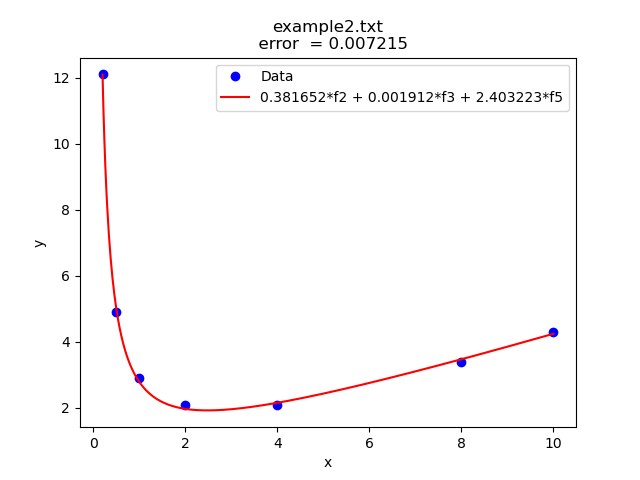
\includegraphics[width=80mm]{C:/Program_Code/NumMeth/Class10STU/code/example2.txt/plot_23_example2.txt.png}
\caption{example2.txtでのデータ点と補間関数(model=23)}
\label{ex2}
\end{figure}

図\ref{ex2}ではデータセットexample2.txtをモデル23($=a_1x+a_2x^2+a_3\frac{1}{x}$)で補間したグラフになる。
この図を見るとデータ点に対してかなり正確な精度で補間出来ていることが分かる。

またerrorの値を見てもほかのモデルが20-0.1程度であるのに対し0.007とかなり小さく収まっていることがわかる。
ただモデル10($=a_1x+a_2\frac{1}{x}$)も誤差が0.007程度に収まっており、モデル23での$x^2$の係数もかなり
小さいことから、場合や用途によっては$x^2$の項を無視したモデル10を用いてもよいかもしれない。

\newpage
\subsection{nh\_bb\_age\_length.txt}
続いてデータセットnh\_bb\_age\_length.txtで最小二乗法を行った結果を図\ref{len}に示す。
\begin{figure}[h]
\centering
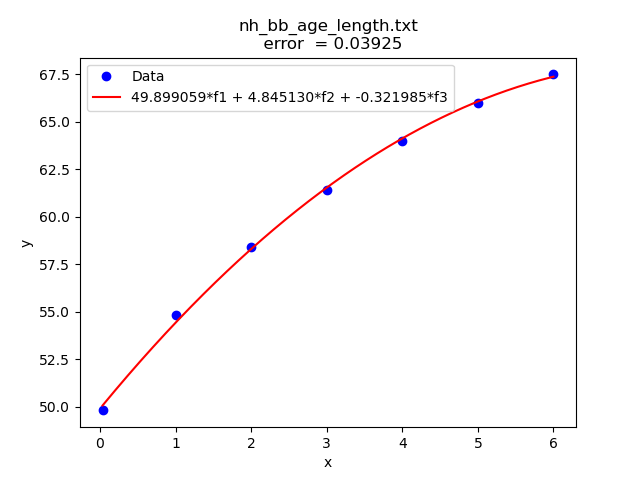
\includegraphics[width=80mm]{c:/program_code/NumMeth/Class10STU/code/nh_bb_age_length.txt/plot_18_nh_bb_age_length.txt.png}
\caption{nh\_bb\_age\_length.txtでのデータ点と補間関数(model=18)}
\label{len}
\end{figure}

図\ref{len}ではデータセットnh\_bb\_age\_length.txtをモデル18($=a_1+a_2x+a_3x^2$)で補間したグラフになる。
この図でもかなり正確な補間ができていることが分かる。

またerrorの値も小さくほかのモデルで行った際は1000-0.1ほどの誤差が出ており、このモデルでの無視出来るほど
小さな係数も存在しないので、今回調べたモデルの中ではこのモデルでの補間が最適であると考える。

このデータセットは名前を見る限り乳児期から幼少期にかけての身長に関するデータであるため、この結果より二次関数で
近似できることが分かる。

\subsection{nh\_bb\_age\_weigth.txt}
続いてデータセットnh\_bb\_age\_weigth.txtで最小二乗法を行った結果を図\ref{wgh}に示す。
\begin{figure}[h]
\centering
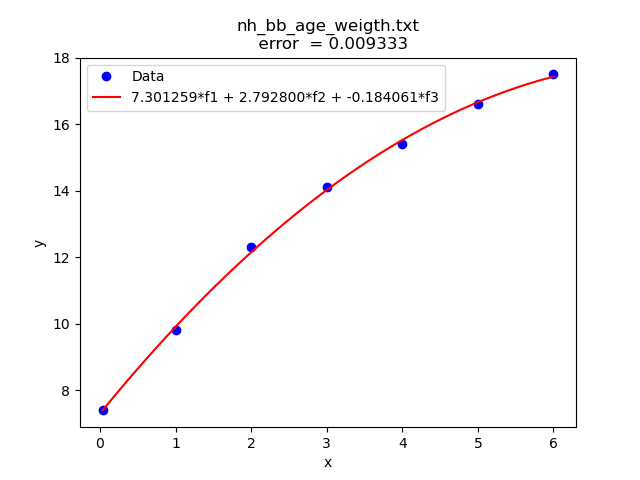
\includegraphics[width=80mm]{c:/program_code/NumMeth/Class10STU/code/nh_bb_age_weigth.txt/plot_18_nh_bb_age_weigth.txt.png}
\caption{nh\_bb\_age\_weigth.txtでのデータ点と補間関数(model=18)}
\label{wgh}
\end{figure}

図\ref{wgh}ではデータセットnh\_bb\_age\_weigth.txtをモデル18($=a_1+a_2x+a_3x^2$)で補間したグラフになる。
この図でもかなり正確な補間ができている。

この補間に関してもerrorが小さく、ほかのモデルでは90-0.03までの誤差が出ており、2.2同様このモデルでの補間が最適であると考えられる。

このデータセットは2.2同様に乳児期から幼少期にかけての体重に関するデータであると思うので、
実際にそういった統計が必要の際には二次関数での補間で都合がよくなると分かる。

\subsection{nh\_covid-italy.txt}
続いてデータセットnh\_covid-italy.txtで最小二乗法を行った結果を図\ref{cov}に示す。
\begin{figure}[h]
\centering
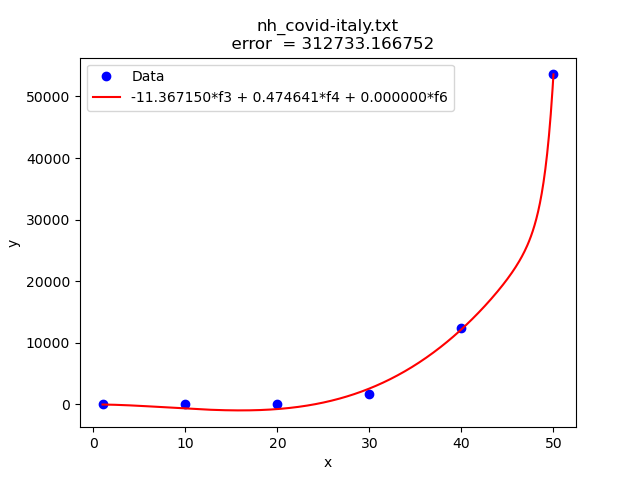
\includegraphics[width=80mm]{c:/program_code/NumMeth/Class10STU/code/nh_covid-italy.txt/plot_26_nh_covid-italy.txt.png}
\caption{nh\_covid-italy.txtでのデータ点と補間関数(model=26)}
\label{cov}
\end{figure}

図\ref{cov}はデータセットnh\_covid-italy.txtをモデル26($=a_1x^2+a_2x^3+a_3e^x$)で補間したグラフになる。
引き続きこの図でも正確な補間ができていることが分かる。

この補間は2.1-3に比べると誤差の値が$3.1 \cdot 10^6$と大きいが、このデータセットでのほかのモデルと比較すると
ほかのモデルは$10^9-10^7$までかなり広い範囲に大きな数字で誤差が出ていることが分かるのでこれが最適なモデルであることが分かる。

このデータセットはこれも名前から予想するにイタリアでのコロナ感染者のデータになっていると思うが、
よく言われている伝染病の感染者数は指数関数的に増加するという言葉通り、項に指数関数が含まれている(係数はかなり小さいが)
のでかなり面白い分析になっていると思う。

\subsection{nh\_fish.txt}
続いてはデータセットnh\_fish.txtで最小二乗法を行った結果を図\ref{fish}に示す。
\begin{figure}[h]
\centering
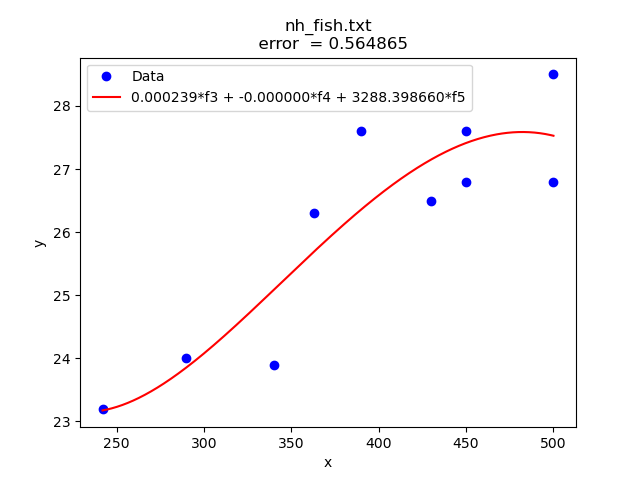
\includegraphics[width=80mm]{c:/program_code/NumMeth/Class10STU/code/nh_fish.txt/plot_25_nh_fish.txt.png}
\caption{nh\_fish.txtでのデータ点と補間関数(model=25)}
\label{fish}
\end{figure}

図\ref{fish}はデータセットnh\_fish.txtをモデル25($=a_1x^2+a_2\frac{1}{x}+a_3e^x$)で補間したグラフになる。

このデータセットはデータ点自体がかなりバラバラであるため図を見ただけでは良い補間になっているかは分からない。
errorの値をほかのモデルと比較してみても15-0.6の付近、特に誤差が0.6付近になるモデルは7つあり、実際にこのデータ
がこのモデルの関係性を持つとは言い切れないような補間になっている。

\subsection{nh\_wine.txt}
最後にデータセットnh\_wine.txtで最小二乗法を行った結果を図\ref{wine}に示す。
\begin{figure}[h]
\centering
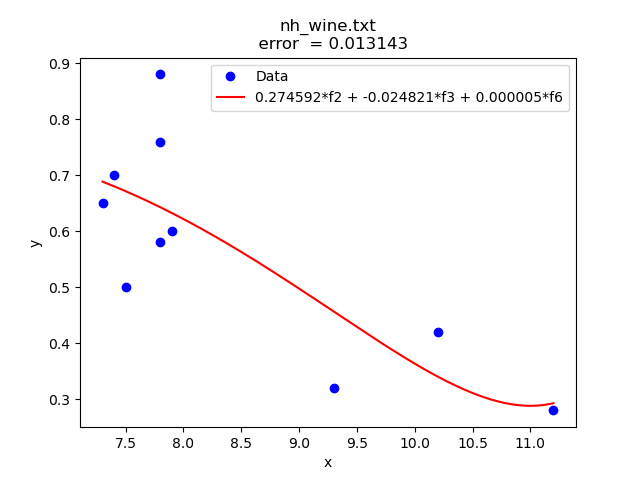
\includegraphics[width=80mm]{c:/program_code/NumMeth/Class10STU/code/nh_wine.txt/plot_24_nh_wine.txt.png}
\caption{nh\_wine.txtでのデータ点と補間関数(model=24)}
\label{wine}
\end{figure}
図\ref{wine}はデータセットnh\_wine.txtをモデル24($=a_1x+a_2x^2+a_3e^x$)で補間したグラフになる。

このデータセットもグラフを見るだけではデータ点により近いような補間になっているとは考えずらい。
errorの値もモデルの半分以上が0.013ほどであり一概にこのモデルが一番良いとは言えない結果であると考えられる。

\newpage
\lstinputlisting[caption=minjijo\_lusolve\_extended.h, label=min.h]{C:/Program_Code/NumMeth/Class10STU/code/minjijo_lusolve_extended.h}
\lstinputlisting[caption=minjijo\_lusolve\_extended.c, label=min.c]{C:/Program_Code/NumMeth/Class10STU/code/main_lusolve_extended.c}
\lstinputlisting[caption=my\_library\_v3.h, label=my.h]{C:/Program_Code/NumMeth/Class10STU/code/my_library_v3.h}
\lstinputlisting[caption=fig.py, label=py]{C:/Program_Code/NumMeth/Class10STU/code/fig.py}
\end{document}